\documentclass[aps,pre,twocolumn,letterpaper,floatfix,showpacs]{revtex4}
\usepackage{graphicx} 
\usepackage{amsmath,amssymb,amsfonts} 
\usepackage{mathtools}
\usepackage{pdfpages}
\usepackage{afterpage}
\usepackage[hidelinks]{hyperref} 
\usepackage{epstopdf}
\usepackage{siunitx}
\usepackage{color}
\definecolor{Blue}{rgb}{0.1,0.1,1.0} 
\definecolor{Magenta}{rgb}{1.0,0.1,0.5} 
\definecolor{LRed}{rgb}{0.8,0.0,0.0} 

 \newcommand{\todo}[1]{ {\color{Magenta} TODO: \color{Blue} \textbf{#1} }}


\begin{document}
\title{Structural replication of nanoporous media using procedural noise}
%\author{A. Hafreager, N. Groeneboom, A. Malthe-S\oe renssen$^1$}
\email{anders.hafreager@fys.uio.no}
\author{Anders Hafreager $^{1}$} 
\author{Nicolaas Groeneboom $^{1}$} 
\author{Anders Malthe-S\o renssen $^1$}
\affiliation{$^1$Department of Physics - University of Oslo\\Sem S{\ae}lands vei 24, NO-0316, Oslo, Norway }
\date{\today} 

%%%%%%%%%%%%%%%%%%%%%%%%%%%%%%%%%%%%%%%%%%%%%%%%%%%%%%%%%%%%%%
%%%%%%%%%%%%%%%%%%%%%%%%%%%%%%%%%%%%%%%%%%%%%%%%%%%%%%%%%%%%%%
\begin{abstract} 
New experimental and observational methods of the structure of three-dimensional porous media calls for improved approaches for statistical characterization and the generation of random samples with given statistical properties. 
We have developed a method for producing statistically consistent realization of porous media using procedural noise functions. By using procedural noise, we are not restricted to generating media with a predetermined resolution, since the noise functions is continuous on all scales. It is therefore possible to generate fractal-like geometries at arbitrary scales. This method is extremely fast and has low memory footprints, requiring very little computational power. We demonstrate the use of procedural noise functions by choosing a method to measure the structural properties of nanoporous media that are created either through regular methods (e.g. molecular dynamics) or with our method. The radial distribution function $g(r)$ is chosen as a measure of the structural properties to compare the simulated geometry to our model. Using this measure, we define a full likelihood framework for estimating model parameters given any data set, and continue by validating our own framework by analysing procedural noise data sets with known input parameters. Finally, we generate a nanoporous media with an expand-and-quench technique using molecular dynamics and show that our model correctly reproduces several of the internal properties of the data set, including $g(r)$, porosity and surface area. 
\end{abstract} 
 
\maketitle
 
% %%%%%%%%%%%%%%%%%%%%%%%%%%%%%%%%%%%%%%%%%%%%%%%%%%%%%%%%%%%%%
%% %%%%%%%%%%%%%%%%%%%%%%%%%%%%%%%%%%%%%%%%%%%%%%%%%%%%%%%%%%%%
\section{Introduction}

The rapid development of new experimental and observational methods to determine the three-dimensional
structure of many types of porous media calls for new statistical tools and methods to characterize
complex porous media and to generate synthetic media based on the observed structures.
New experimental methods allow for studies of three-dimensional structures from nano-meter to meter scales.
Destructive techniques such as focused ion beam scanning electron microscopy (FIB-SEM) are routinely
used to characterize geologically relevant structures in shales and carbonate rocks with resolutions
down to tens of nanometers \cite{cnudde2013high,curtis2010structural}.
High-energy X-ray tomography methods using high-energy beams at international research facilites or
in-house scanners open for three-dimensional mapping of mineral structures from sub-micrometer to
millimeter scales \cite{kobchenko20114d,jamtveit2014pore,zhu2011microtomography,fusseis2009creep}.
Thus new experimental techniques provide three-dimensional voxelized images that can form the basis
of analysis or modeling.
However, in many cases we can only scan a few examples experimentally, but need to perform simulations
over many statistically similar realizations to find effective properties or to populate upscaling models.
Thus the need for methods to robustly characterize three-dimensional porous structures and to generate
synthetic structures with similar statistical properties. 

The field of synthetic rocks is a large field both scientifically and technologically \citep{biswal2007stochastic,hamzehpour2006development, yeong1998reconstructing}. 
Methods to generate synthentic rock samples from experimental characterizations may be based on 
purely statistical or geometrical models, models of physical processes that generate the samples, or combinations of both. 
For small-scale porous media, physical models are often used to generate initial grain
packings \cite{pilotti1998generation,scott1969density,herrmann2013physics}, then further mechano-chemical
and fluid-mediated processes such as precipitation-dissoluton processes and pressure
solution \cite{rutter1983pressure}, or fracture and plastic deformation processes are added
to include effects of long-term compaction \cite{rutter1983pressure,renard1997pressure}. 
On large scales, reservoir models are populated by statistical models for lithological and
geomorphological processes \cite{pyrcz2014geostatistical}, such as river fan formation to
generate particular grain size distributions \cite{koltermann1996heterogeneity,blair1994alluvial}. 
More statistical approaches include variations of percolation models \cite{sahimi} or
network models \cite{fatt1956network,sahimi1993flow} to characterize and generate uncorrelated or correlated porous media. 
In addition, the high resolution of observational methods allow three-dimensional scans to
form the basis for atomic-scale modeling using molecular modeling methods such as
molecular dynamics or Monte Carlo methods to study the dynamics of nanoporous media. 
But then procedural or physical models are needed to fill in the atomic scale details, to
build many statistical realizations of nanoporous media with atomic-scale details, and to extrapolate to larger scale models.

These physically based models may not always include all relevant effects, can be quite
computationally expensive when used to generate many samples, and cannot easily be extended
beyond the initial size of the simulated systems. 
For example, to prepare a simulation of nanoporous silica, we need to carry out a sequence
of large scale simulations in molecular dynamics, which is time consuming, computationally
expensive and the results cannot be exteded beyond the intial size of the simulated systems
without performing another simulation \cite{Adarsh}. 
On the other hand, the statistical models often do not include all the correlations induced
by physical processes or have limited number of tunable parameters. 
In particular, statistical models have challenges in reproducing atomic-scale structures of nanoporous media. 


Meanwhile, there has been a recent growth in advanced random noise models that open for new
ways to generate structured noise with statistical similarities to real samples, such as the use of Perlin noise. 
Such noise models have been used to model systems with complex statistical correlations such
as in GAMER\cite{groeneboom:2014}, and show great promise in being adaptable to many different physical systems. 
Also, such noise models are continuous and extendable, so that arbitrary large systems or
systems with arbitrary high precision can be modeled. 
While these models show great promise in several fields \cite{ebert2003texturing, cook2005wavelet, bridson2007curl, goldberg2008anisotropic},
they have not yet been systematically applied to characterize or generate nanoporous media with statistical properties corresponding to that of real systems.

In this paper, we propose a new method for producing realistic-looking nanoporous media
using only random noise fields, without the need for physics simulations. 
We provide a systematic study of the use of procedural noise-based models to characterize
and generate three-dimensional nanoporous media. 
Our studies will be based on silica-based nanoporous media, for which we have good atomic
scale models and physics-based methods to generate porous media as a sequence of simulated
processes, and we therefore can generate large-scale samples where we have full knowledge of all aspects of the material. 
These simulated systems are then characterized using the radial distribution function, $g(r)$,
statistical methods are generated with similar properties, and compared with the simulated systems. 
Using these approaches we find that procedural noise methods can be tuned to efficiently create
materials that are structurally similar to simulationed materials. 

\section{Procedural content generation}
By procedural content generation, we generally mean a mathematical algorithm that uses limited
input data to create complex, sometimes infinite repeating patterns.
A firm example would be fractals, such as the Julia/Mandelbrot [ref Mandelbrot] set, where one
tests whether the complex quadratic recurrence equation $z_{n+1} = z_n^2 +C$ for $z \in \mathbb C$
converges for each position in a 2D complex plane.
With this seemingly simple equation, the level of complexity generated on the boundary between
convergence and divergence is infinite, with self-similar patterns repeating themselves to arbitrary detail.

Another example, widely used in contemporary game content generation, is having prefabs, or
pre-fabricated 3D models such as doors, walls, tiles and roof segments automatically being
stitched together to create buildings.
When designing a city, instead of creating each building manually, you only need specify the
position, area and height of a structure.
Then, by using an algorithm that combines these prefabs to render the building, it is possible
to create cities of arbitrary size with a single command.
Naturally, it is also possible to create procedural methods that design the layout and placement of these buildings.

A much simpler example would be generating a 1 (or 2)-dimensional terrain by choosing random
points on a grid and performing a spline interpolation between them to create the illusion of a smooth landscape.
In fact, this is the very essence of procedural noise, which we are focusing on in our model,
and the first person to create such a fast algorithm for N-dimensional spline interpolation
between pseudo-random points was Ken Perlin\cite{perlin1985image}.

\subsection{Perlin/Simplex noise}
\label{sec:perlin}

Procedural algorithmic methods for creating realistic-looking
fractal-like patterns have been around for more than 30 years. The most famous of these
algorithms is Perlin noise, first developed by Ken Perlin in 1983 for
use in the movie ``Tron''\cite{perlin1985image}. 

Perlin noise is a type of pseudo-random gradient noise that mimics a Gaussian field, but at low computational cost.
An improved version of Perlin noise is called simplex noise, which has several advantages
over standard Perlin noise in terms of scalability and speed \cite{perlin:2002}.
Perlin noise was developed in response to the lack of detail 1980's contemporary graphics,
where polygonal surfaces often were bland and left without any detail.
In response to this problem, Perlin noise was developed in order to continuously perturb
the light bouncing off flat surfaces, effectively yielding bump mapping and producing a much more realistic image.

An overview of the current state of procedural noise functions can be
found in \cite{lagae2010state}. Perlin noise is a band limited repeatable pseudo-random function
from $\mathbb R^n \to \mathbb R$ that is computationally fast, and has
properties which make it suitable for creating patterns that mimic
nature. Perlin noise is an approximation to Gaussian filtered noise
implemented as a pseudo-random spline. The algorithm uses a predefined
grid of gradients pointing in a random direction, where for any point
within a grid, we interpolate the gradients from the four corners. The
algorithm is as follows:
\begin{itemize}
  \item[1.] For a point, obtain the four closest gradients in the grid.
   \item [2.] For each of the gradients, calculate the dot product
     between the gradient and a vector defined by the  the distance
     between the the point and the current grid corner. 
   \item [3.] Instead of linear interpolation $F(t) = t$, use a fade function to produce
   smoother interpolated values. Perlin noise typically uses the following fade function: $F(t) = t ^3 (t  (6 - 15) + 10)$.
    \item [4.] Obtain the final value by linearly interpolating between the x-axis and
      use this result to linearly interpolate the y-axis. 
\end{itemize} 
Simplex noise works in a similar manner, but works on on simplices instead of hypergrids,
and so requires fewer computational steps, scales better in higher ($\ge 3$) dimensions
and has fewer anisotropic properties. 

\subsection{Properties of Perlin/simplex noise}
\begin{figure}
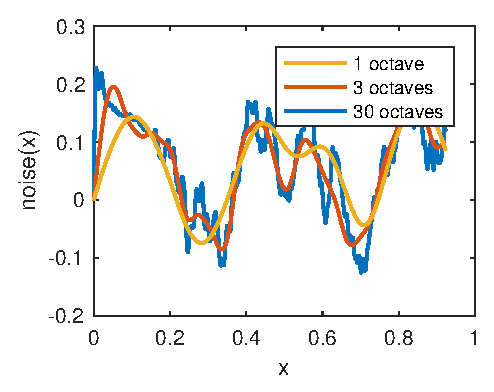
\includegraphics[width=.5\textwidth]{noise.eps}
\caption{Perlin noise (left) versus simplex noise (right). Note the
  straight x-y pattern in the single upper Perlin mode and the less
  anisotropic simplex mode. Lower part: combining octaves tend
  to remove these patterns.}
\label{fig:noise}
\end{figure}

\begin{figure}
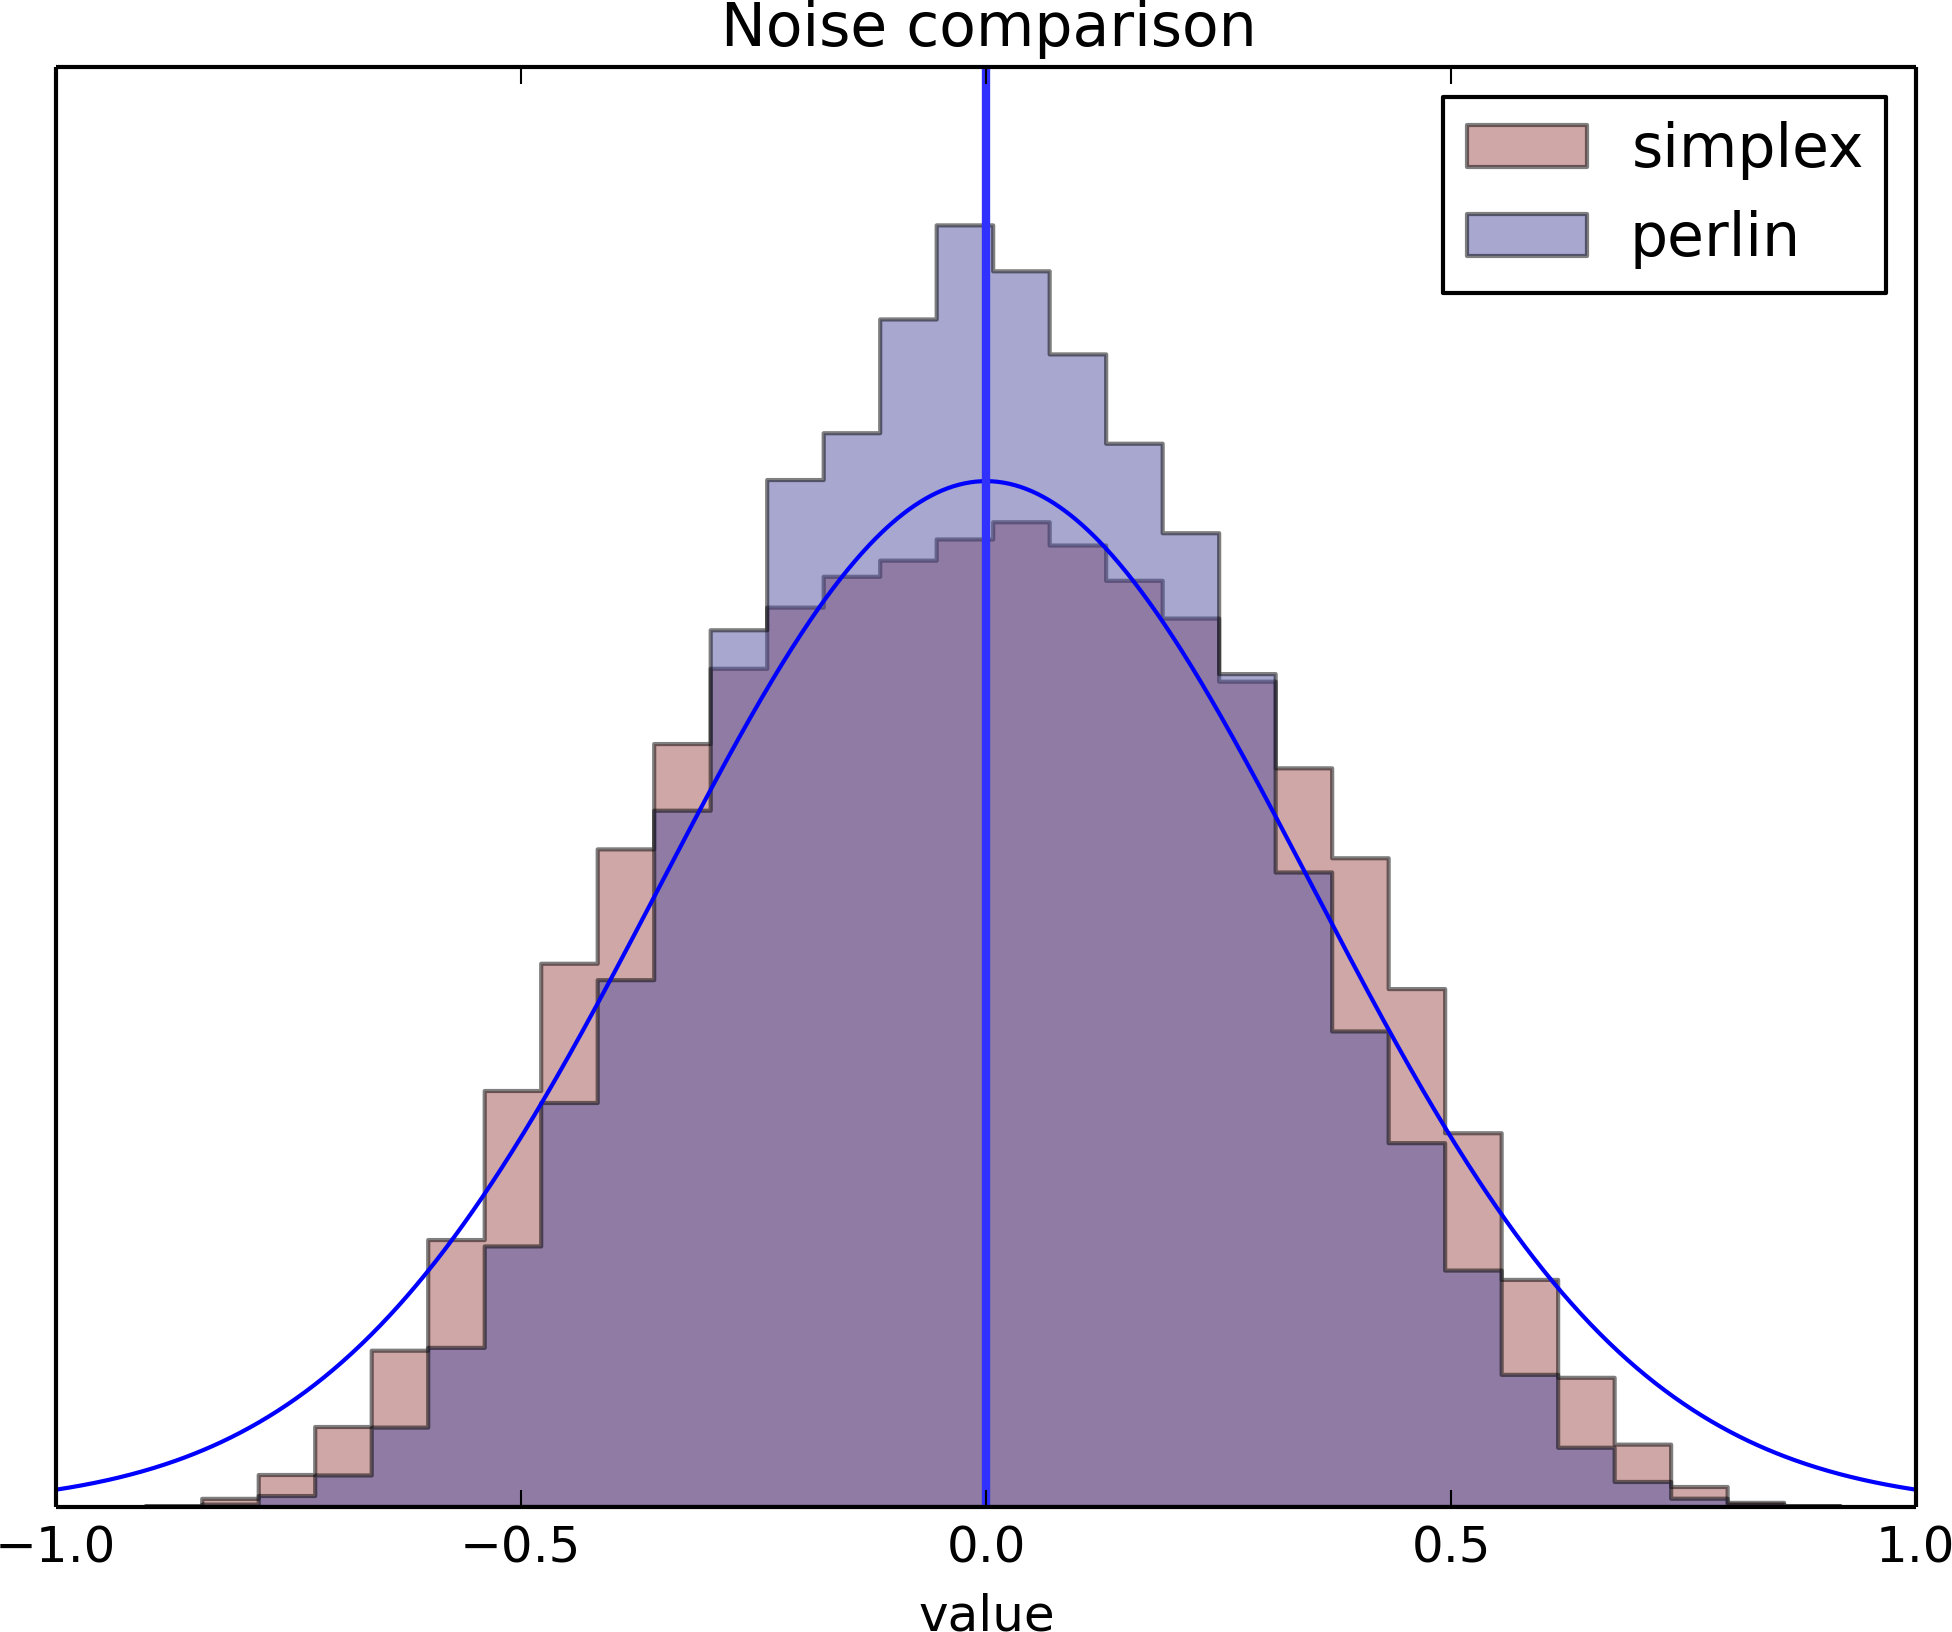
\includegraphics[width=.5\textwidth]{noise_comparison.png}
%\mbox{\epsfig{file=perlinstats.eps, width=\linewidth}}
\caption{Normalized distributions of Perlin noise and simplex noise compared with a
  Gaussian distribution. Note how both noise functions produce
  near-Gaussian, but slightly different distributions.}
\label{fig:properties}
\end{figure}
Standard Perlin noise is known for having several anisotropic features
\citep{lagae:2010}. Perlin noise also gives rise to a ``textile''
pattern in the $x$ and $y$-directions, which is evident from the upper
left part of figure \ref{fig:noise}, depicting 2D Perlin noise in
a single octave. The upper-right part shows the same node for simplex noise,
with less obvious ``textile'' features. However, when combining several octaves
and adding a random shift to the coordinates, as depicted in the two lower parts,
these anisotropic patterns tend to cancel
out.  In addition, we have calculated the statistical distributions for Perlin and simplex noise
with $\sigma = 0.35$, and have plotted the results in figure \ref{fig:properties}.
Each procedural noise method has distributions that are close to normal, 
but with some asymmetrical properties. 


\subsection{Multiple octaves: creating patterns}
\label{sec:octaves}
The different octaves from procedural noise functions can be combined
to produce a wide range of nature-like patterns. A generic
$N$-dimensional procedural function $\Phi(\vec x): \mathbb R^N \to
\mathbb R$ could be expressed as
\begin{equation}
\label{eq:procedural}
 \Phi(\vec x) = \Theta \Big(\sum_k^\Omega \kappa (k) P(  f_s (\vec x,k) )) \Big),
 \end{equation}
where $f_s(\vec x,k)$ describes the frequency scale modifier (e.g. $f_s(\vec x,k) =
k\vec x$), $\Omega$ is the amount of octaves (modes), $\kappa(k)$ is the octave amplitude (e.g. $\kappa(k) = 1/k$)
and $\Theta(x)$ an overall modifier (e.g. $\Theta(x) = x$ or
$\Theta(x) = \frac{1}{x}$). In a sense, $\kappa(k)$ is similar to Fourier coefficients. 
In its simplest case, summing directly over the octaves with amplitude $1/k$ results in 
\begin{equation}
\label{eq:perlinlinear}
 \Phi(\vec x) = \sum_k^\Omega \frac{1}{k} P( 2k\vec x).
\end{equation}
In one dimension, we show equation \ref{eq:perlinlinear} with 1, 3 and 30 octaves
in figure \ref{fig:1dperlin}, while the 2D procedural noise pattern is depicted in the lower
part of figure \ref{fig:noise}. Finally, since simplex noise both scales better
with higher dimensions and produces less asymmetric effects, we choose to use
simplex noise over regular Perlin noise as the main noise function throughout this paper.

\begin{figure}
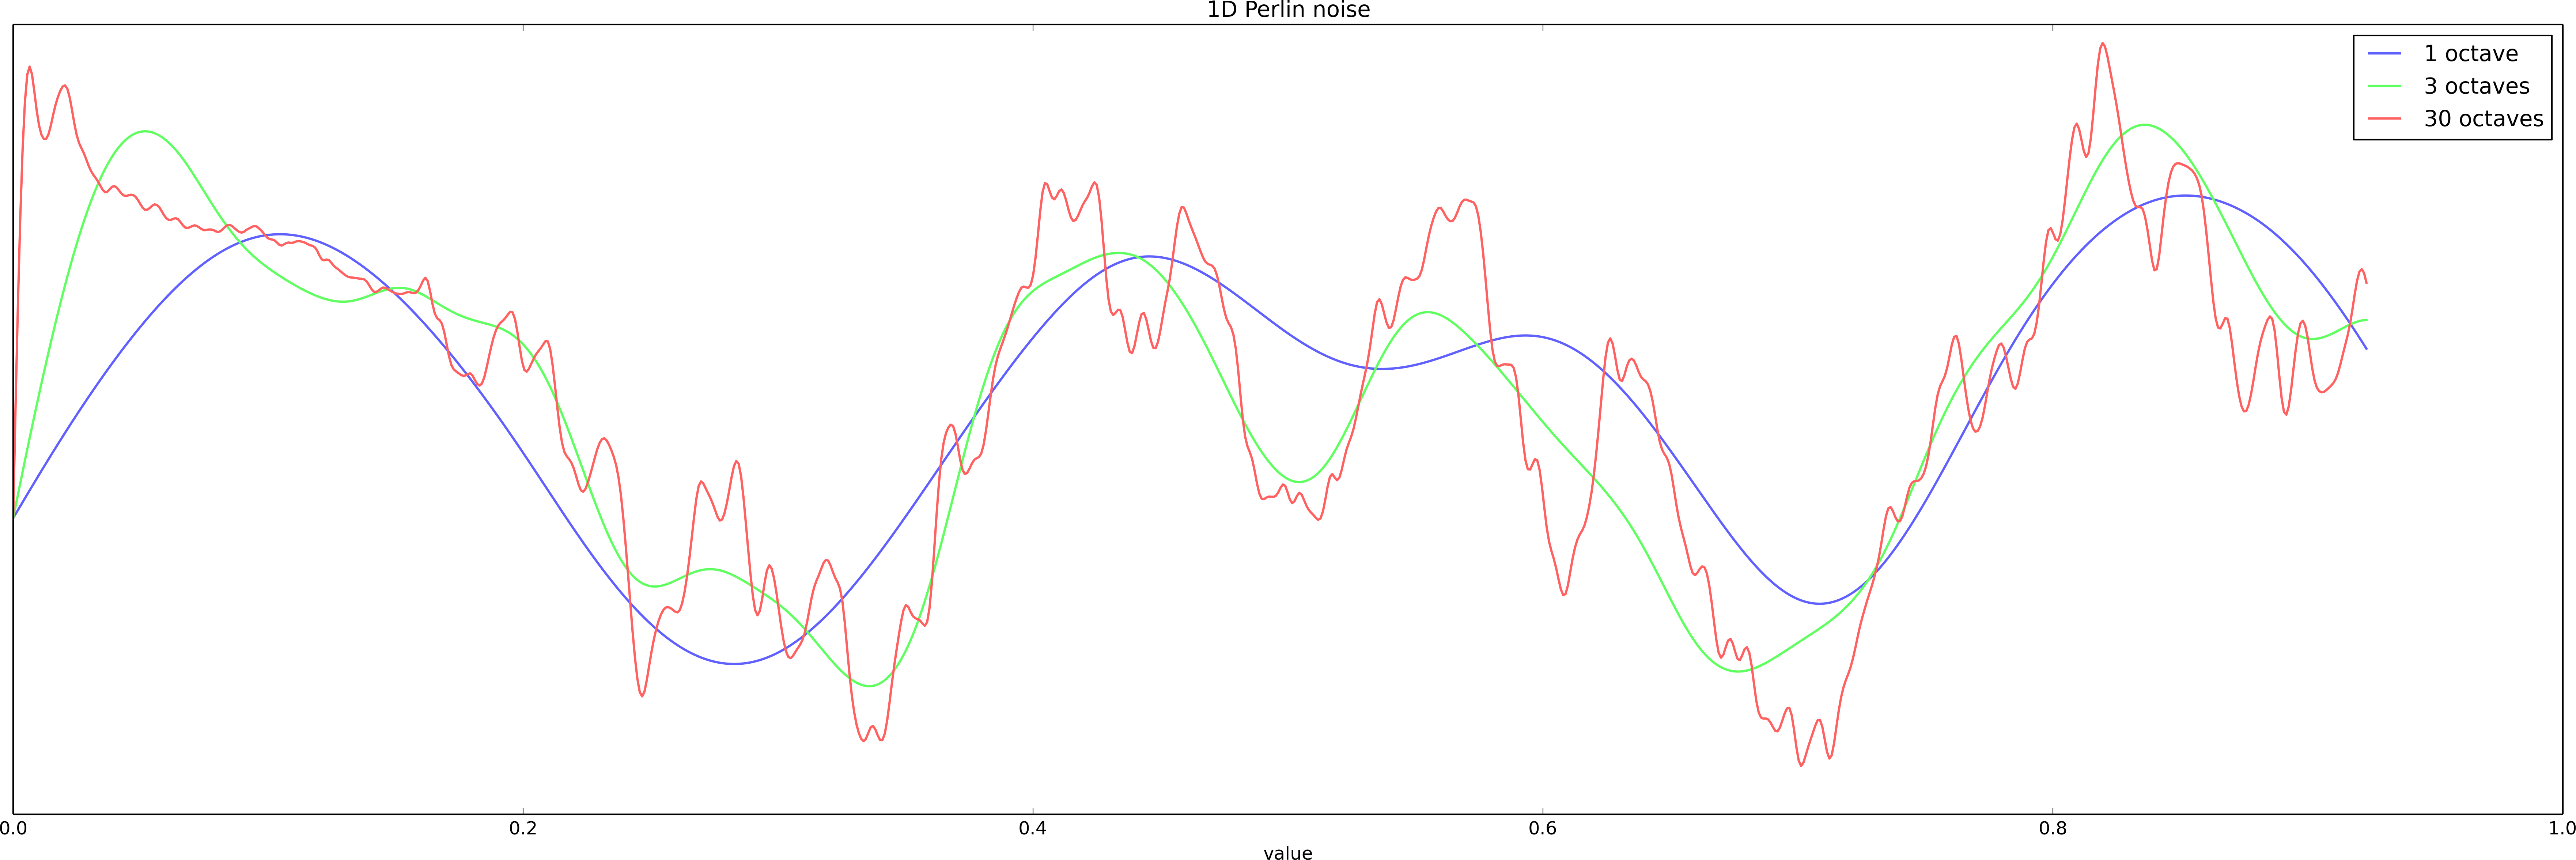
\includegraphics[width=.5\textwidth]{1d_perlin.png}
\caption{1D simplex noise with 1 (blue), 3 (green) and 30 (red) octaves. }
\label{fig:1dperlin}
\end{figure}


\section{Model}
In this paper, we are interested in developing a model using simplex noise to reproduce
nanoporous structures that are statistically similar to physical simulations of porous media.
For a given data set and a model, we wish to estimate the parameters that best represent the data. 
This is performed through a full likelihood analysis in order to obtain the posterior
probability distribution of the parameters. 
The model measure of the analysis is the radial distribution function $g(r)$, for
which the parameters will be adjusted to maximise.
In addition, we also investigate the porosity and surface area of the system. 
The simulated system is confined to a cube of size $\SI{159} {\angstrom}^3$, but since
the procedural noise function is continuous on all scales, the box could be of arbitrary size. 

\begin{figure*}
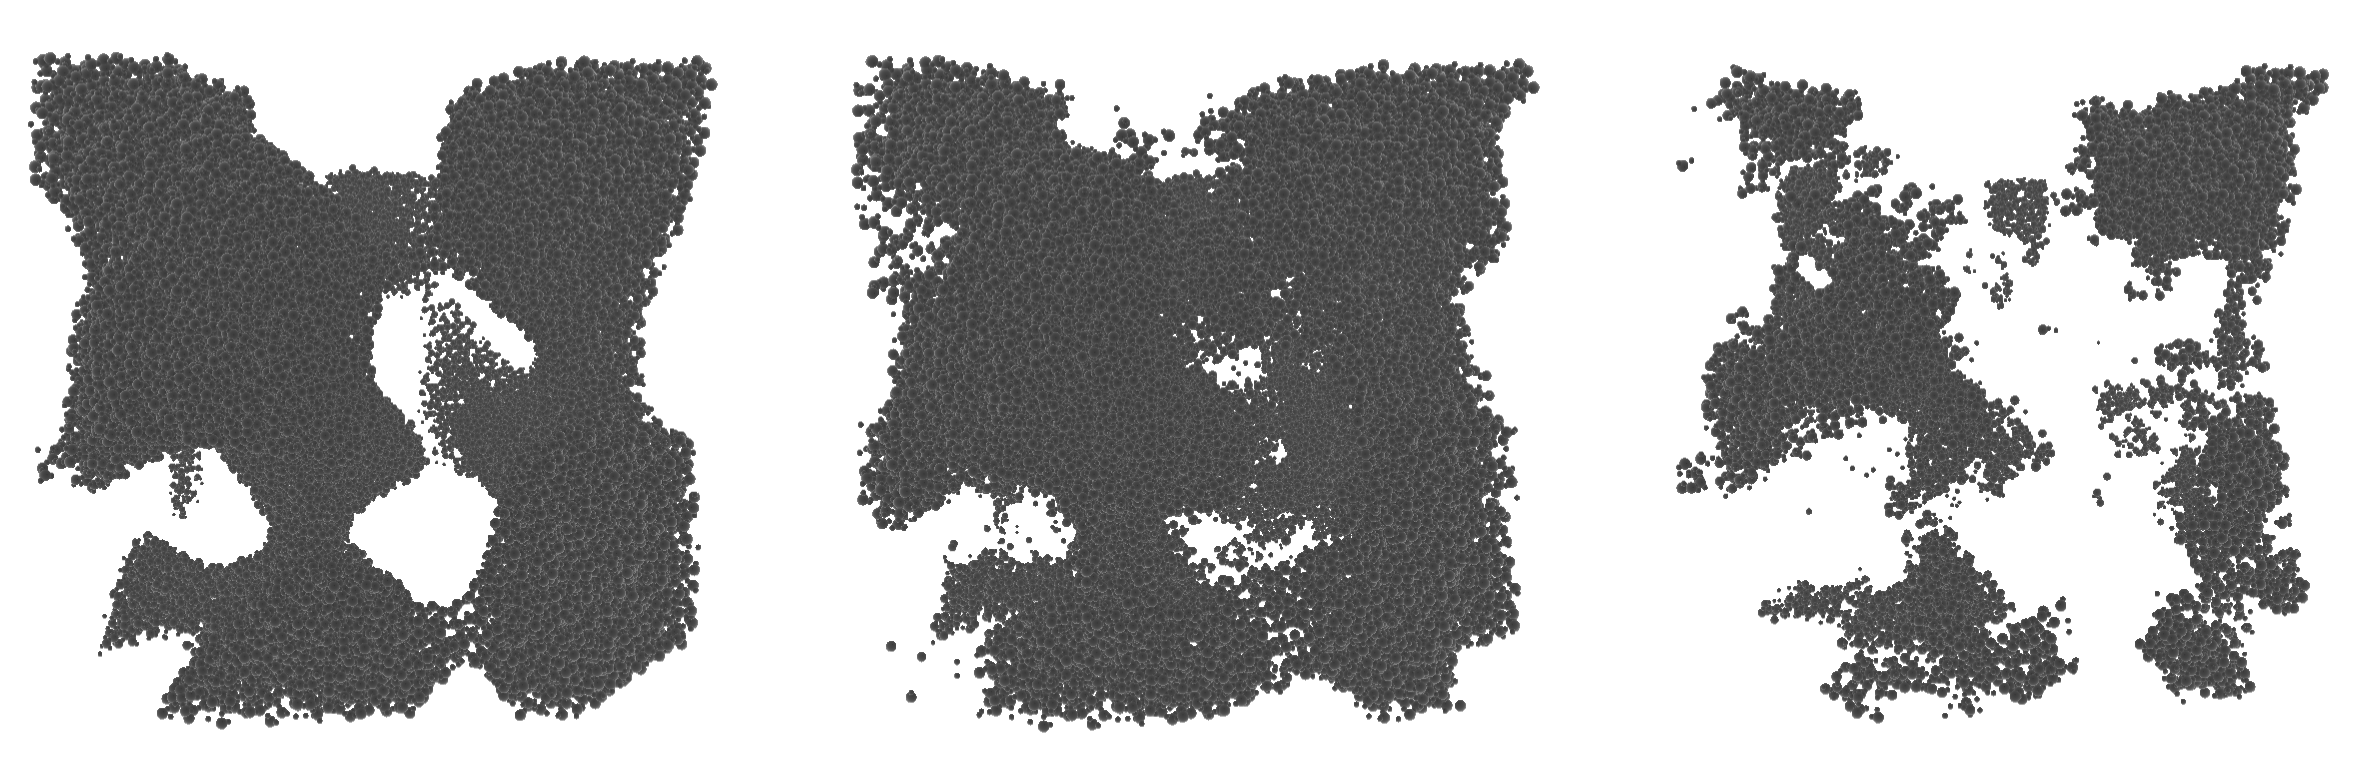
\includegraphics[width=.95\textwidth]{model_examples.png}
\caption{Examples of 3D simplex noise structures in nanoporous media. Left image:
low persistence (large scale dominates), middle image: medium persistence (small
scales starts dominating) and right image: high threshold (more atoms are discarded). }
\label{fig:model_example}
\end{figure*}
We construct a generic sum over procedural noise octaves with the expression: 
\begin{equation}
  M_1(\bar \theta) = M_1(\vec x, \psi, \Omega, \nu) = \sum_{\omega=0}^{\Omega} \psi^{\omega -1}   N\big((\vec x + \vec\sigma \cdot \omega)\nu \cdot 2^{\omega-1} \big),
\label{eq:noisemodel1}
\end{equation}
where $\Omega$ is the number of octaves, $\psi$ the persistence (scale falloff),
$N$ a generic $N$-dimensional noise function, $\vec \sigma$ a predefined random
vector that removes anisotropic artefacts and $\nu$ the frequency modifier representing
the initial largest scales in the model. For simplicity, $\bar \theta$ here denotes
the set of model parameters. For each mode, the frequency is thus multiplied, while
the overall amplitude is damped by a given persistence. In the end, we simulate a
large set of bulk particles without any walls, and use the noise function to remove
particles that are not within a procedural void given by a threshold $\tau$. Three
examples of this model are depicted in figure \ref{fig:model_example}, where we have
used $\Omega=6$ octaves and the scale is $\nu=0.01$ and cut-off $\tau=0$. The left
image depicts low persistence ($\psi = 0.0$), where only the first octave dominates
(corresponding to large scales). The middle picture shows the same parameters with
a higher persistence $(\psi = 0.5)$, where smaller scales become more dominating.
In the rightmost picture, the effect of the cut-off threshold $\tau = -0.3$ is shown to emphasize threshold cut-off. 


\subsection{Model Measure}
In order to perform data analysis on the model parameters, we developed a code that
uses Monte Carlo Markov chains to produce samples for building the posterior probability distribution for the parameters. 
Before doing so, we need a model measure - a quantitative method that characterizes
the internal structure of the porous media. This quantity should be computed for both
the original data set and the one produced by our noise model. 

Ideally, the model measure should pick up all geometrical properties that are
relevant for the physical study of interest. 
For instance, transport in porous media heavily depends on the pore size
distribution and porosity, whereas chemical reactons are sensitive to surface area \cite{coussy2011mechanics}.
In this paper, we choose to focus on the radial distribution function (RDF)
$g(r)$ as defined and implemented in LAMMPS \cite{plimpton1995fast}.
$g(r)$ describes how density varies as a function of distance from a 
reference particle, picking up both the intramolecular and intermolecular structure. 
We have chosen to ignore the short range contributions of $g(r)$ since
the pore geometry does not depend on the intra-molecular structure of
SiO$_2$, but only the density variations at larger distances. 
Hereafter, $g_d(r)$ denotes the RDF calculated from simulated or experimental data,
while $g_{M(\bar \theta)}(r)$ represents the RDF based on the procedural noise
model $M(\bar \theta)$, where $\bar \theta$ is the set of model parameters. 

The method used for calculating porosity of a media is defined as in \cite{gelb1998characterization},
and we obtain the surface area of a porous media by using m arching cubes triangulation to sum the
surface area of the generated triangles.
As discussed in \cite{gelb1998characterization}, the definition of surface area is ill-defined in
atomic simulations, because a clear definition of pore space is needed. 
In the marching cubes triangulation, we create a voxelized grid, a scalar field with values being
the distance from the voxel centre to the nearest atom. 
The isovalue threshold defining the surface is chosen to be \SI{2}{\angstrom}, large enough to
contribute to a dense pore matrix, but small enough to have most of the available pore space defined as such. 
The important note here is that the same definition of both surface and porosity is being used
in all systems that are compared, physical simulations, procedural methods or data. 

\todo{skriv litt mer om hvorfor vi velger g(r)}


%\begin{figure}[htb!]
%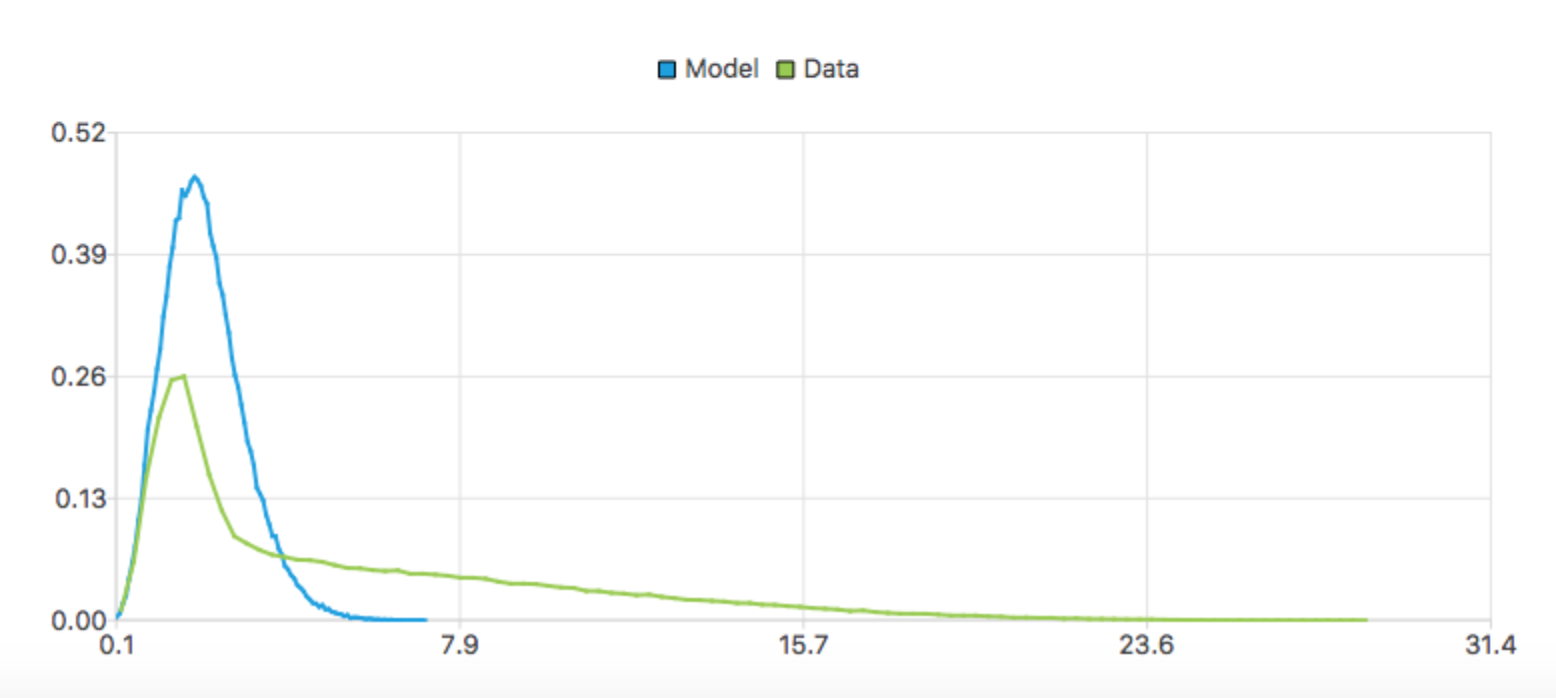
\includegraphics[width=.45\textwidth]{DTA.png}
%\caption{Distance-to-atom measure for two data sets with varying persistence. The green line corresponds to a mock data set with low persistence (dominated by large-scale modes), while the blue line corresponds to high persistence (dominated by small scale modes). }
%\label{fig:dta_example}
%\end{figure}



%\subsubsection{Fractal Dimension}
%The fractal dimension is a ratio providing a statistical index of complexity comparing how detail in a pattern changes with the scale at which it is measured. We provide a fracal

%\subsubsection{Octree Counting Measure (OCM)}

%\subsection{Diffusion Measure}

\subsection{Data analysis and the Likelihood}

The posterior probability distribution is defined as the probability of the parameters
$\bar \theta$ given the evidence $d$, or $P(\bar \theta | d)$. Bayes' theorem states that 
\begin{equation}
P(\bar \theta | d) = \frac{P(d | \bar \theta)P(\bar \theta)}{P(d)} \propto P(d | \bar \theta)P(\bar \theta),
\end{equation}
where $P(d | \bar \theta)$ is called the Likelihood $\mathcal L$ (the probability of
evidence given parameters) and $P(\bar \theta)$ is the prior (the beliefs about the
quantity before some evidence is taken into account). $P(d)$ is called the evidence,
and is the probability of the observations (here assumed to be 1). Prior parameters
are restricted to freely roam within a minimum and maximum value, so we can therefore
assume that the posterior distribution is proportional to the likelihood, or
$P(d | \bar \theta) \propto \mathcal L$. In other words, to calculate the posterior
probability distribution and obtaining the best fit model parameters, we need only
to estimate the likelihood function, which is connected to the $\chi^2$ by 
\begin{equation}
\mathcal L \propto e^{-\chi^2}.
\end{equation}


In order to estimate whether two 3D data sets are statistically equivalent up to
the model measure $g(r)$, we calculate the $\chi^2$ between the two one-dimensional
RDFs. Pearson's $\chi^2$ is defined as 
\begin{equation}
  \chi^2 = \sum_r \frac{ \Big(g_d(r) - g_{M(\bar \theta)}(r) \Big)^2}{g_{M(\bar \theta)}(r)^2},
\end{equation}
so for low values of $\chi^2$, the better the fit between data and model, up to
$g(r)$. For a single-parameter model, we could simply just iterate over the lone
parameter to obtain the minimum $\chi^2$ (where the best-fit parameter value resides),
however, with increased number of parameters comes increased computational cost.
If we divide the parameter space into $N$ bins, the number of $\chi^2$ computations
scales as $N^d$, where $d$ is the number of model parameters. To be able to build
the full landscape of the posterior probability distribution, we need to use the Monte Carlo Markov chain (MCMC) method .

We are now interested in maximising the likelihood $\mathcal L$ as opposed to
minimising the $\chi^2$, with the goal of mapping out the full $d$-dimensional
likelihood space for the model parameters. We build the $d$-dimensional likelihood
by letting random walkers traverse the parameter space guided by the MCMC test:
for each step $M(\bar \theta_{n})$ in parameter space, we calculate the likelihood
$\mathcal L_n$ for this particular parameter configuration. Then, for the next
step, we create a new set of parameters $M(\bar \theta_{n+1})$ by choosing new
parameters randomly from a $d$-dimensional sphere around the previous parameter
composition. The model also selects a new random seed. We calculate the proposed
likelihood $\mathcal L_{n+1}$ at this new step and perform the MCMC test: accept
the new step if $\frac{\mathcal L_n}{\mathcal L_n+1} \ge 1$, or reject if the value
is lower than a uniform random value $\in [0,1]$. 

Finally, we obtain the posterior $P(\bar \theta | d) \propto \mathcal L$ by building
a $d$-dimensional histogram of the likelihood using the stored positions of the parameters.
For a sufficiently large amount of steps, the MCMC algorithm ensures that the posterior
converges to the likelihood, as long at the surface does not contain unreachable areas
such as discontinuous patches or an infinite amount of maxima (as is the case for the
function $f(x)=sin(\frac{1}{x}$). Luckily, as we shall see, the likelihood surface for
our models tend to turn out with a single, well-defined maximum.  


\section{Results}
We now turn our attention to applying the MCMC framework on two kinds of data.
First, we wish to test and verify the code by performing a full data analysis on
mock data with known input parameters. This enables us to investigate the posterior
distribution, and determine whether any potential problems could arise with the
likelihood landscape, such as random walkers trapped in local minima. In addition,
we will obtain an intuition on the width of the estimated parameter distributions.
But most importantly, we will have verified that our likelihood code is working correctly
if we successfully reproduce the original input parameters. We then continue with a
full analysis of simulated SiO$_2$ data, and see whether the resulting best-fit
parameter data set is consistent with the SiO$_2$ data set. 

\subsection{Model verification: Parameter estimation of mock data}
\begin{figure}[htb!]
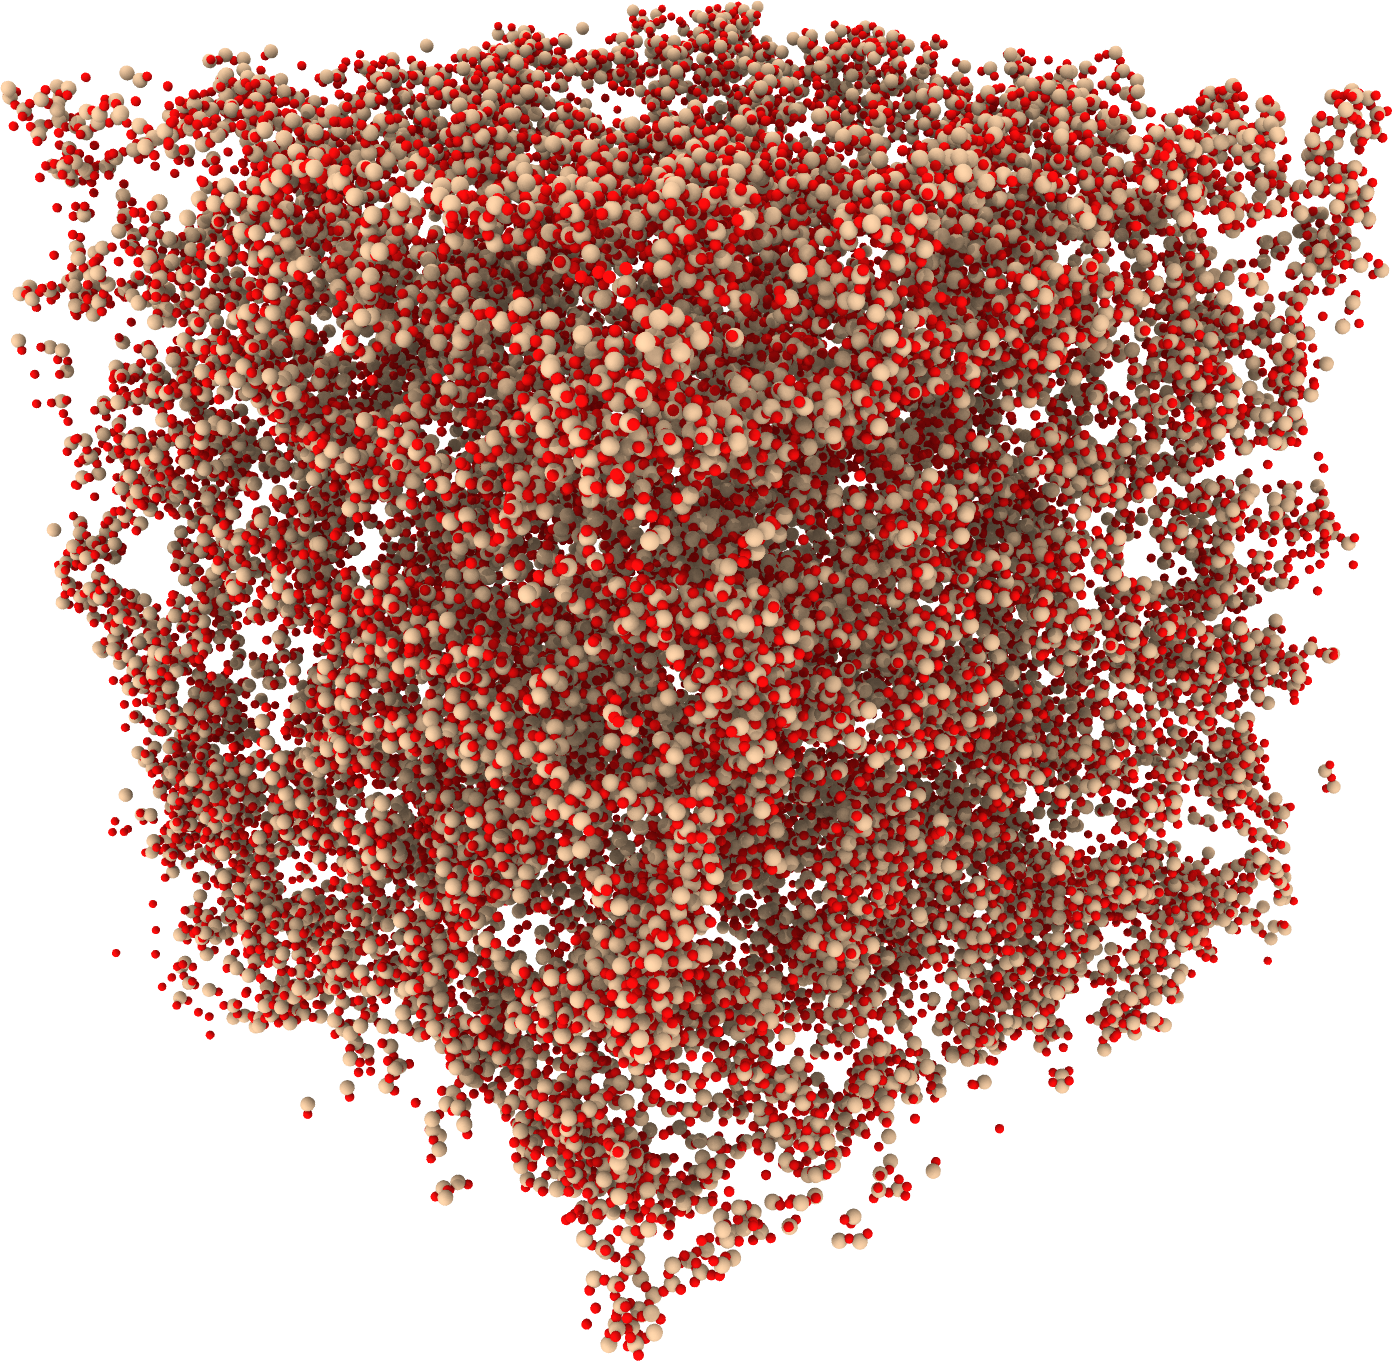
\includegraphics[width=.45\textwidth]{model_test.png}
\caption{Simulated mock data used for the initial model testing analysis. Input parameters are $\nu=0.03$,$\tau=-0.02$ and $\psi=0.6$.}
\label{fig:mockdata}
\end{figure}
In order to verify our likelihood code, we perform a model verification test
on a mock data set with known input values based on equation \ref{eq:noisemodel1}.
In this example, we only use standard simplex noise with three free parameters:
the persistence $\psi$, threshold $\tau$ and scale $\nu$. We simulate a data set
of size $\SI{159} {\angstrom}^3$ with $\sim 255 000$ atoms, and perform the cut-off
given by input parameters $\Omega=3$, $\Psi = 0.6$, $\tau=-0.2$ and $\nu=0.03$.
The resulting 3D structure is depicted in figure \ref{fig:mockdata}. 

We continue by executing a full MCMC analysis on the mock data by using a
parallelized code written in C++ running on a 48 core cluster. About 48 hours
was needed to produce about 300 000 samples. The results from this analysis
can be seen in figure \ref{fig:mockdataresults_pts}, where the upper panel
depicts the marginalised 1D posteriors while the lower shows the marginalised
2D posteriors. The centre and left image shows that the input parameters of
$\tau=-0.2$(threshold), $\psi=0.6$(persistence) and $\nu=0.03$ are all reproduced
well within $1 \sigma$. Note that there seems to be no problems with the posterior
distribution in terms of local minima or multiple maxima. In addition, the results
show that all the parameters are correlated with $r \sim 0.85$, while the width of
the marginalised distributions vary by $\sigma_\tau = 0.02 \sim 10\%$, $\sigma_\Psi = 0.062 \sim 20\%$ and $\sigma_\nu = 0.01 \sim 33\%$. 

\begin{figure*}
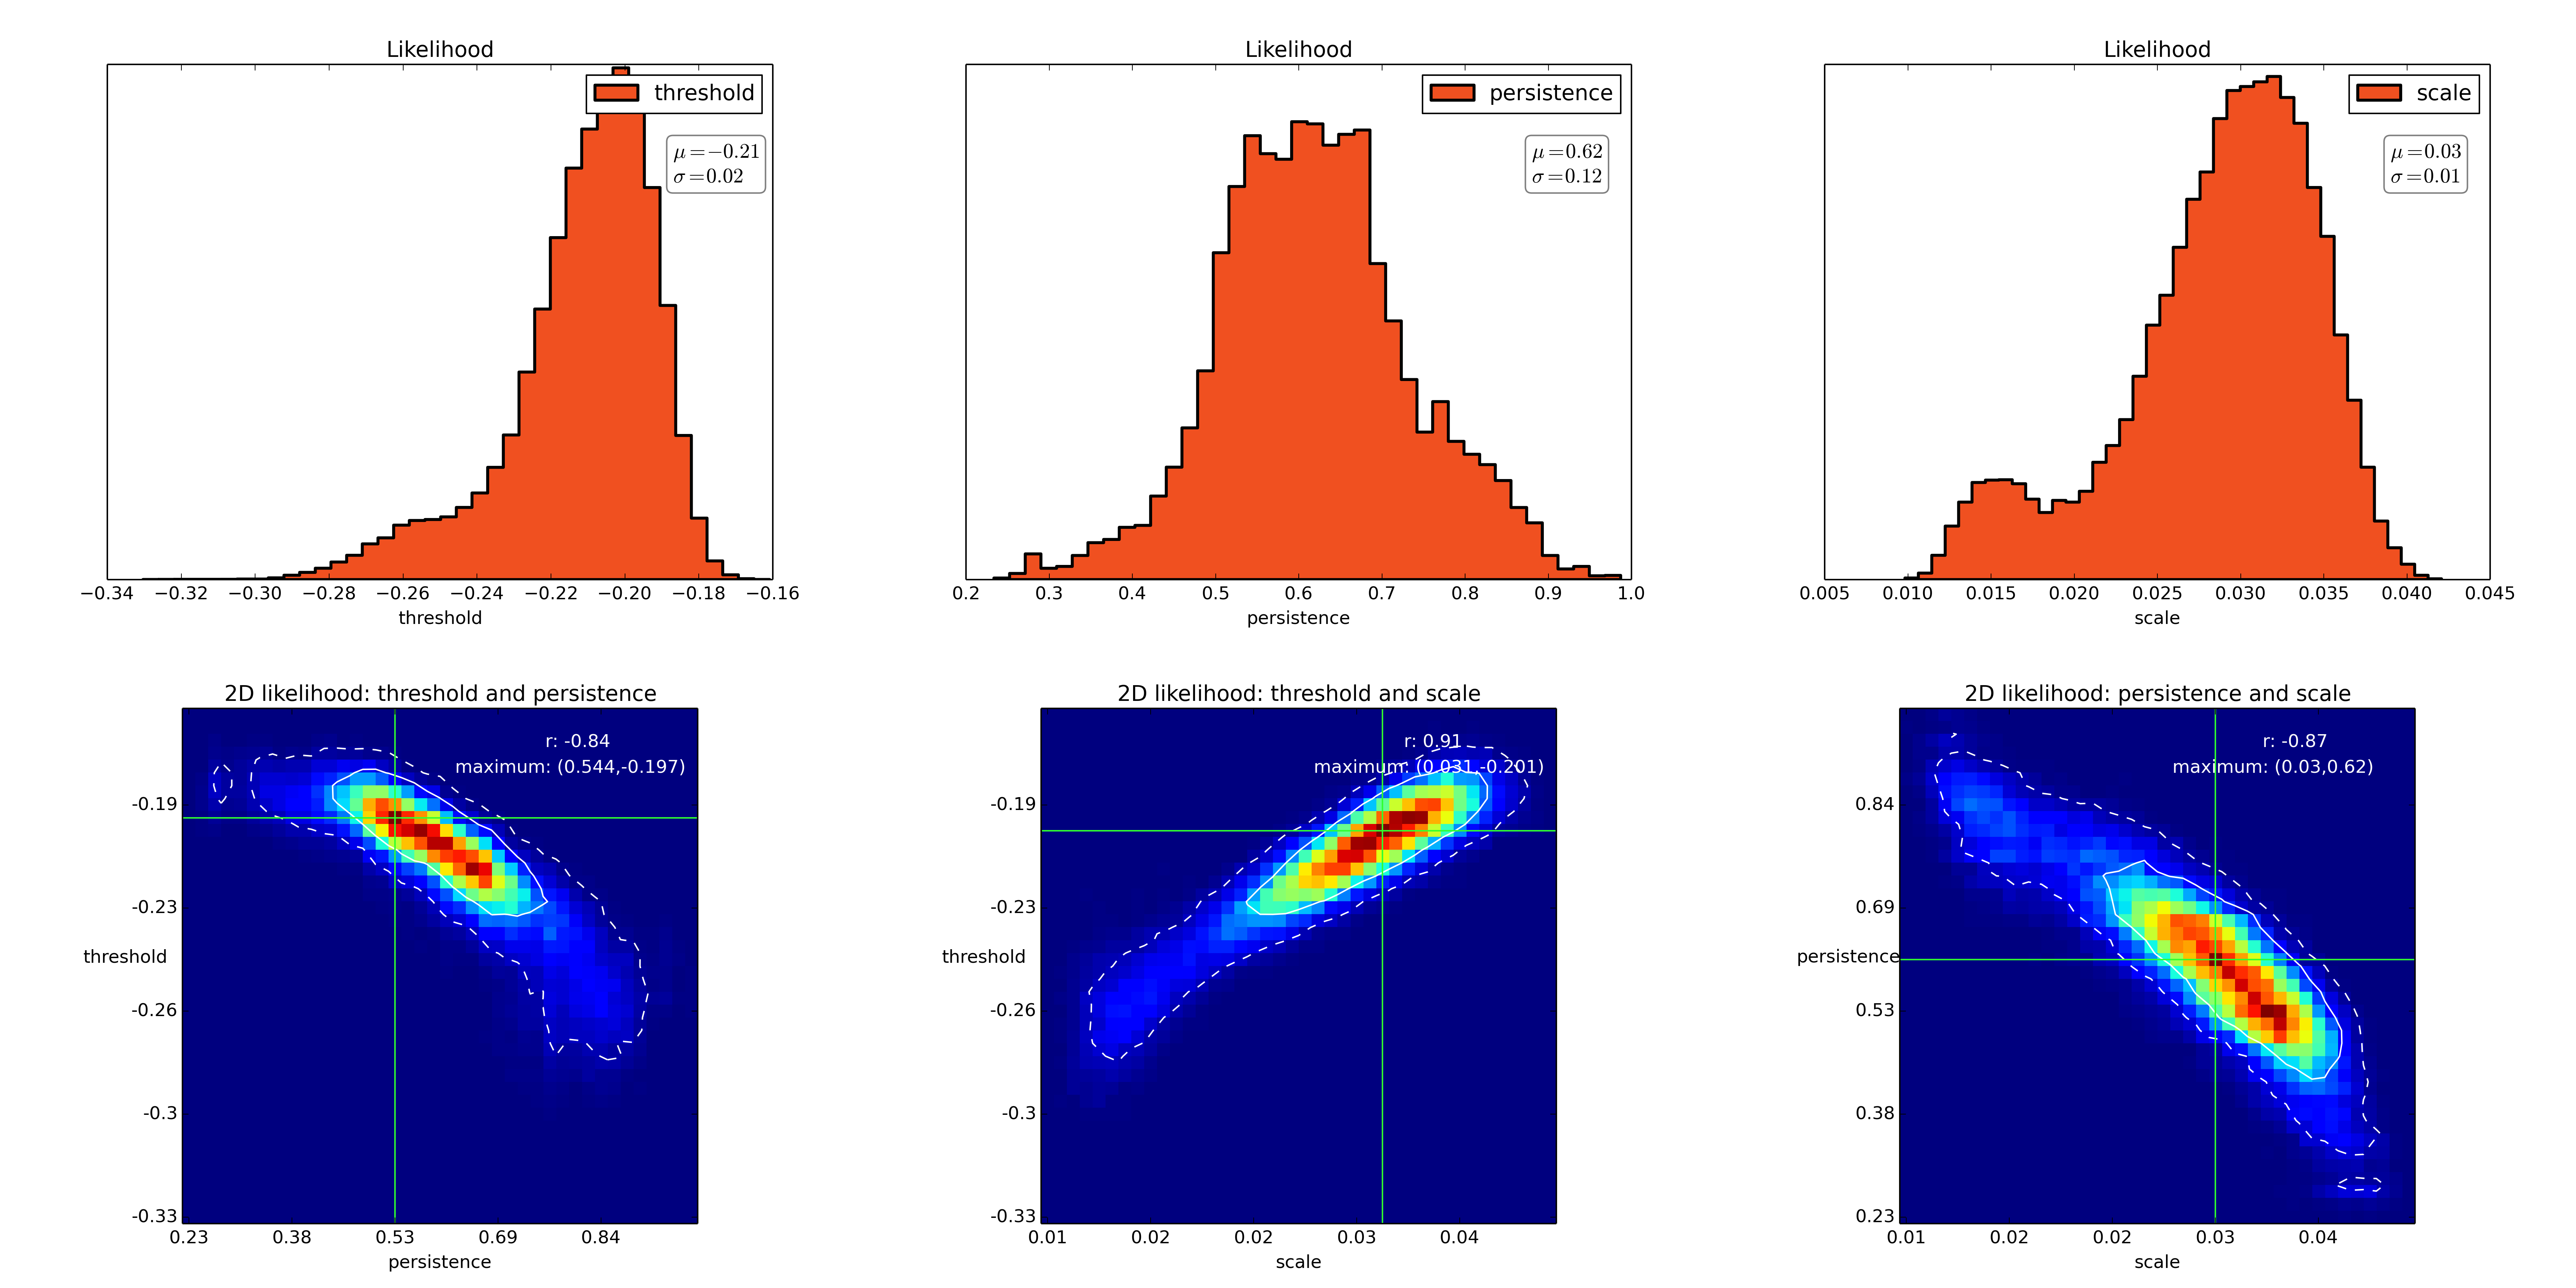
\includegraphics[width=.99\textwidth]{mock_data_results_pts.png}
\caption{Results from the model validation simulation.The upper panel displays the marginalised 1D posteriors for each parameter, while the lower panel depicts the marginalised 2D posteriors. Note that all input parameters were reproduced well within $1 \sigma$ (inner contour line).}
\label{fig:mockdataresults_pts}
\end{figure*}

\subsection{Parameter estimation of simulated nanoporous silica}
%\begin{figure}
%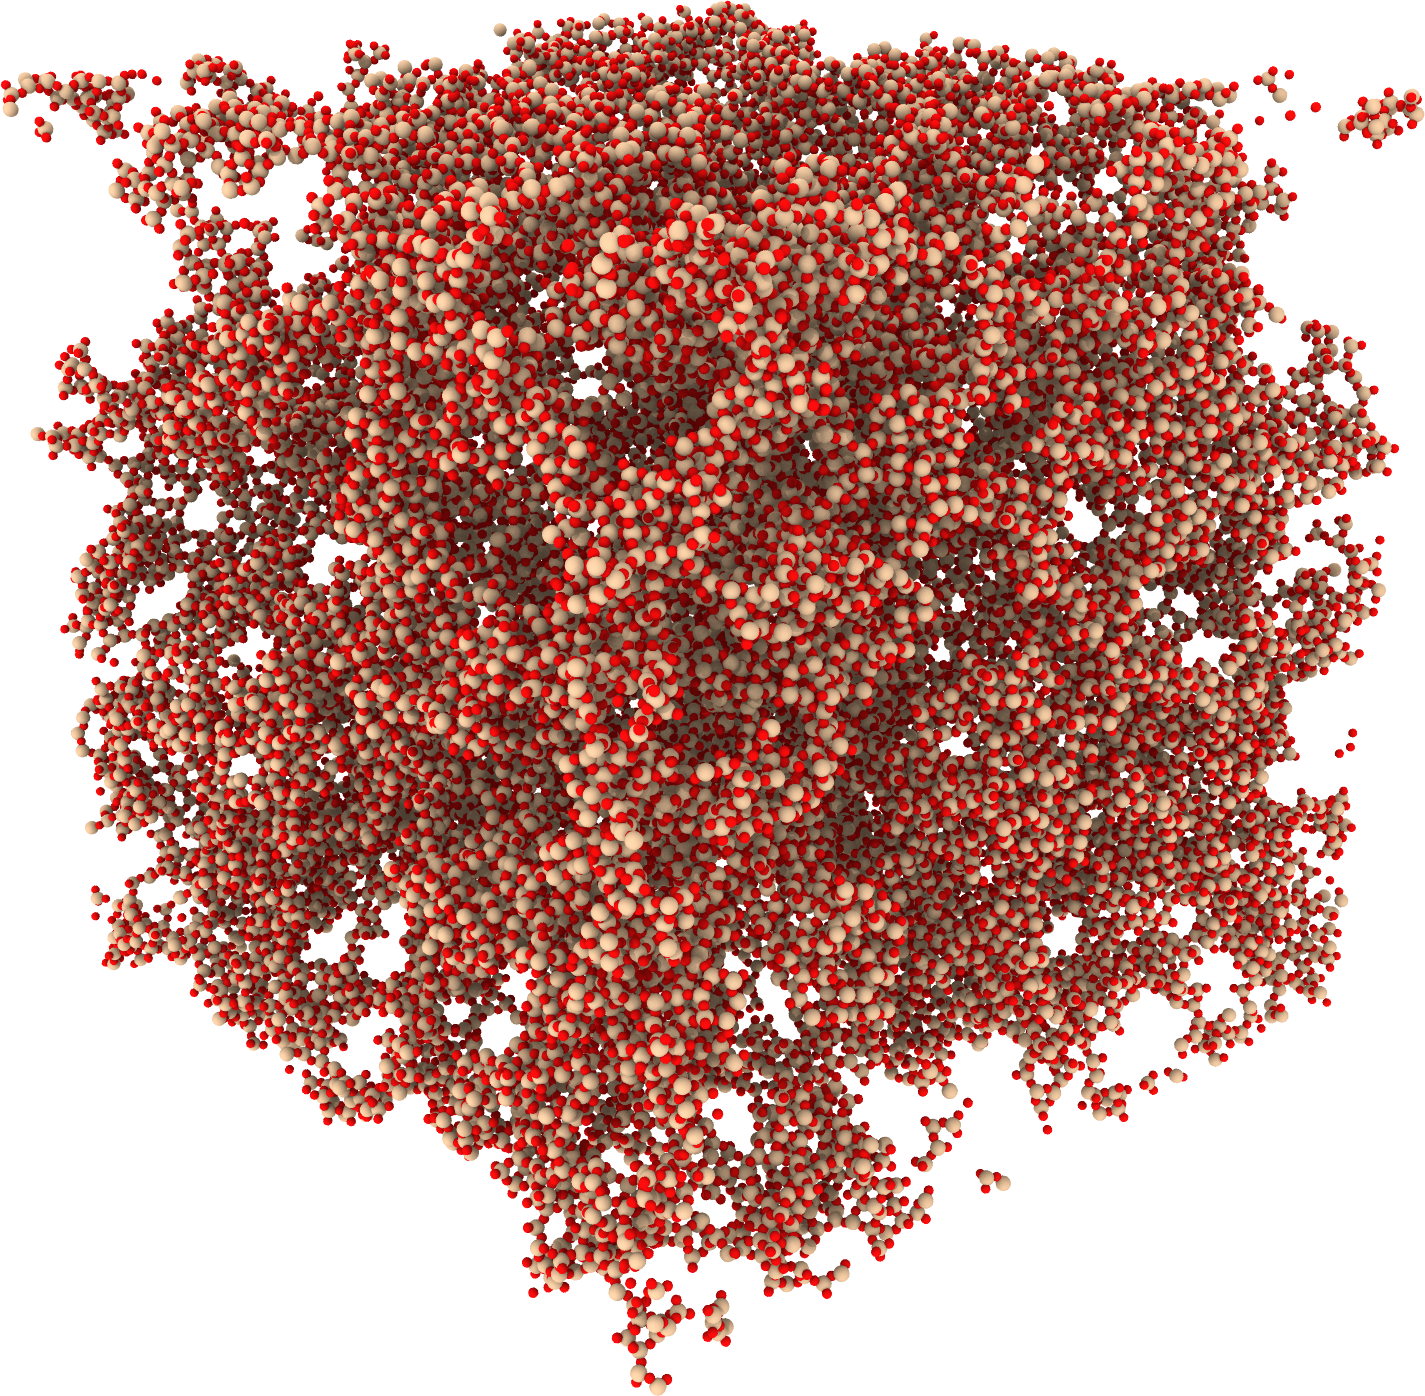
\includegraphics[width=.49\textwidth]{sio_porous.png}
%\caption{Simulated silica created with LAMMPS. The box is $159^3 \AA$, with $100 000$ particles, having been created by cooling an expanding system until quenching was achieved. Note the similarities between the pores here and in figure \ref{fig:mockdata}.}
%\label{fig:si2data}
%\end{figure}
\begin{figure*}
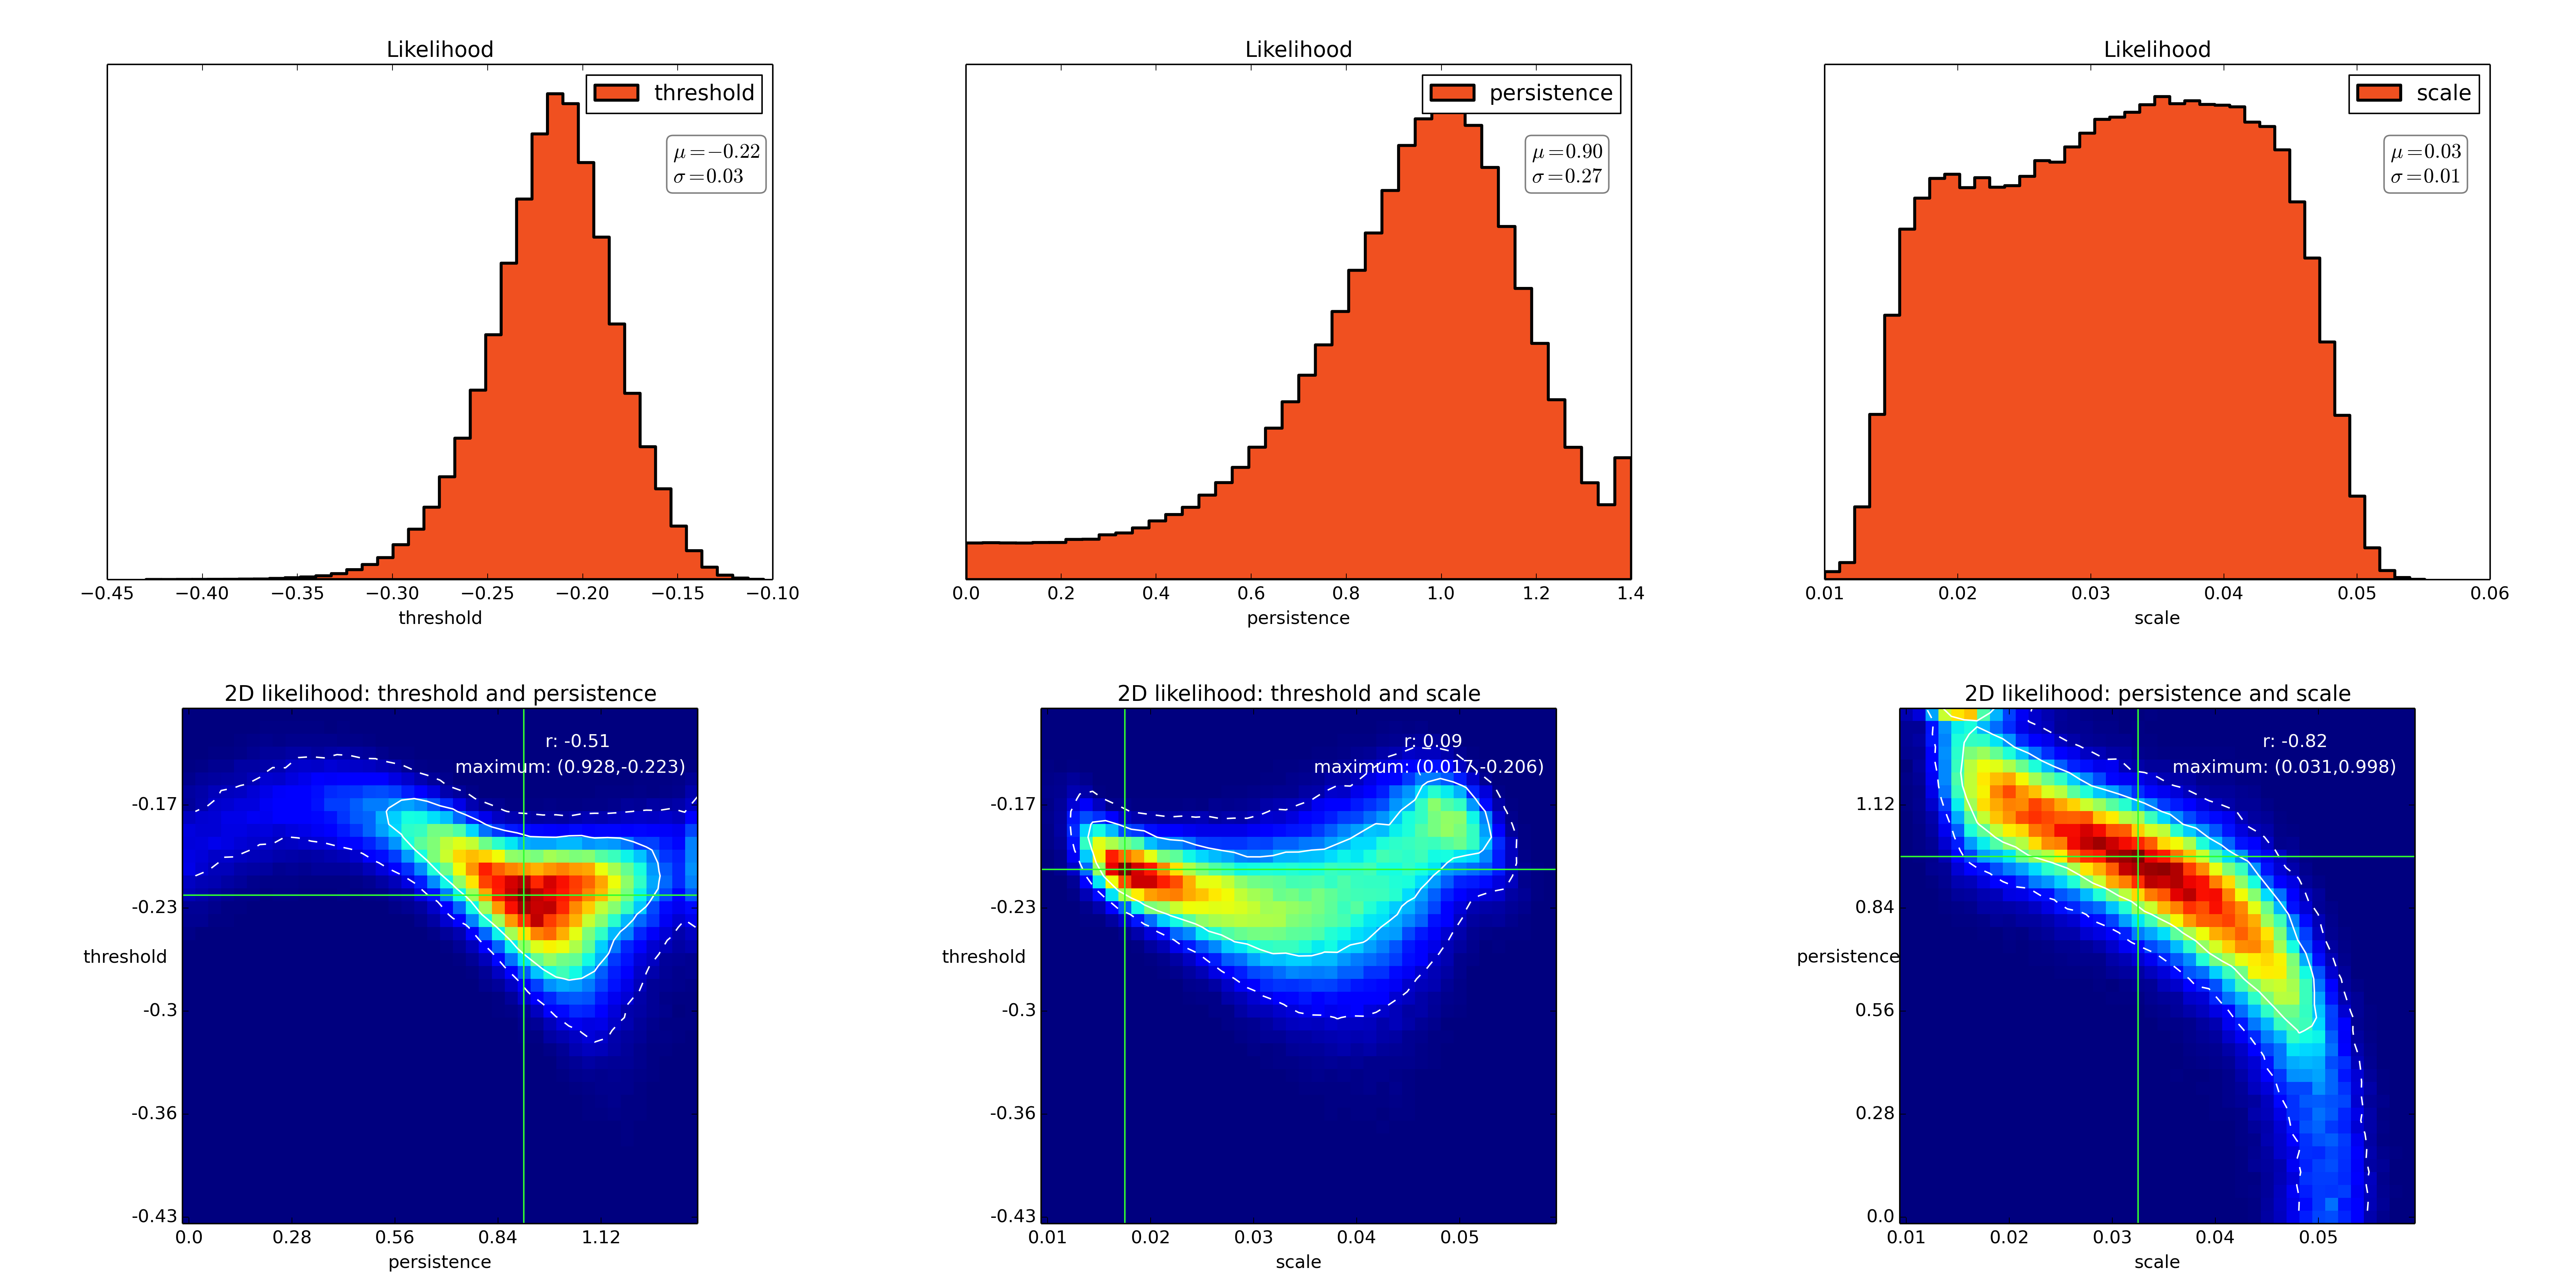
\includegraphics[width=.99\textwidth]{results_porous_full.png}
\caption{
Results from the analysis of a simulated $\SI{159} {\angstrom}^3$ SiO$_2$ nanoporous data set. The upper panel displays the marginalised 1D posteriors for each parameter, while the lower panel depicts the marginalised 2D posteriors. Best fit parameters from the maximum 3D likelihood suggest $\tau=-0.2$, $\psi=0.8$ and $\nu=0.3$.
}

\label{fig:porous_results1}
\end{figure*}
Having verified that the likelihood code yields correct results when analysing mock data, we turn to 
performing a parameter fitting analysis on realistic simulated nanoporous media.
Using LAMMPS \cite{plimpton1995fast} and the Vashishta-potential \cite{vashishta1990interaction},
we simulate system consisting of $14^3$ betacristobalite unit cells of SiO$_2$, corresponding
to system size of approximately \SI{100}{\angstrom}. 
The temperature is then increased to \SI{4500}{\kelvin} using NVT integration. 
After an initial period, we expand the box to \SI{159}{\angstrom} to achieve a porosity $\phi=0.75$. 
Then, the system is quenched by setting the temperature to \SI{300}{\kelvin},
resulting in the nanoporous media on the right side in figure \ref{fig:porous_vs_model}. 
By choosing a different seed for the initial velocities, it is possible to produce
statistically equal samples but with random realizations. 


With the model described in equation \ref{eq:noisemodel1}, we perform a full likelihood
analysis of the data set with the three free parameters $\tau$, $\nu$ and $\psi$ using $g(r)$ as the measure. 
The resulting marginalised posteriors are depicted in figure \ref{fig:porous_results1},
where the best-fit parameters $\tau=-0.2$, $\psi=0.8$ and $\nu=0.3$ is extracted from the full 3D likelihood. 
We also display $g(r)$ for the input data set, a best-fit parameter data set and a
bad-fit data set in figure \ref{fig:gofr1}, to illustrate the sensitivity of $g(r)$ given the model parameters. 
Note that we are not able to accurately reproduce the structures of the SiO$_2$ $g(r)$ with
our current model, but hope that we during future work will be able to produce another model
that provides a better fit with this measure. 
\todo{skriv om hvorfor vi ikke plukker opp alle features?}

Note that the surface atoms are not in chemical equilibrium since some neighbours of a surface atom might have been removed. 
In order to use the generated geometry in molecular dynamics, one would need either noble gas
atoms which may be stable, or to apply passivation step.

\begin{figure}
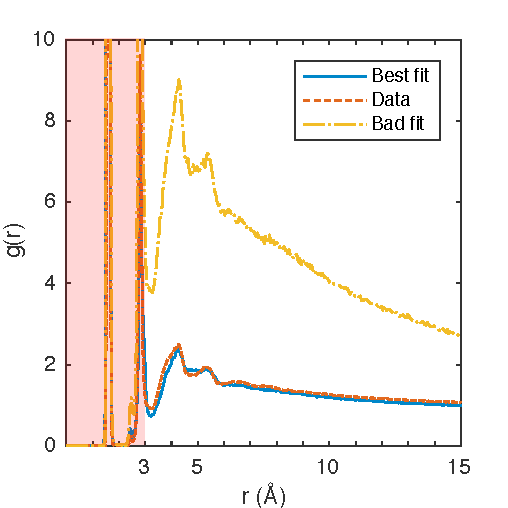
\includegraphics[width=0.5\textwidth]{gofr_figure.pdf}
\caption{$g(r)$ for three data sets: the simulated SiO$_2$ input data set (red), the best-fit parameter model (blue) and a random low-fit parameter model (green).}
\label{fig:gofr1}
\end{figure}
Finally, we depict a comparison of the actual simulated input SiO$_2$ data set together with a
representation of the best-fit parameters in figure \ref{fig:porous_vs_model}   
\begin{figure}
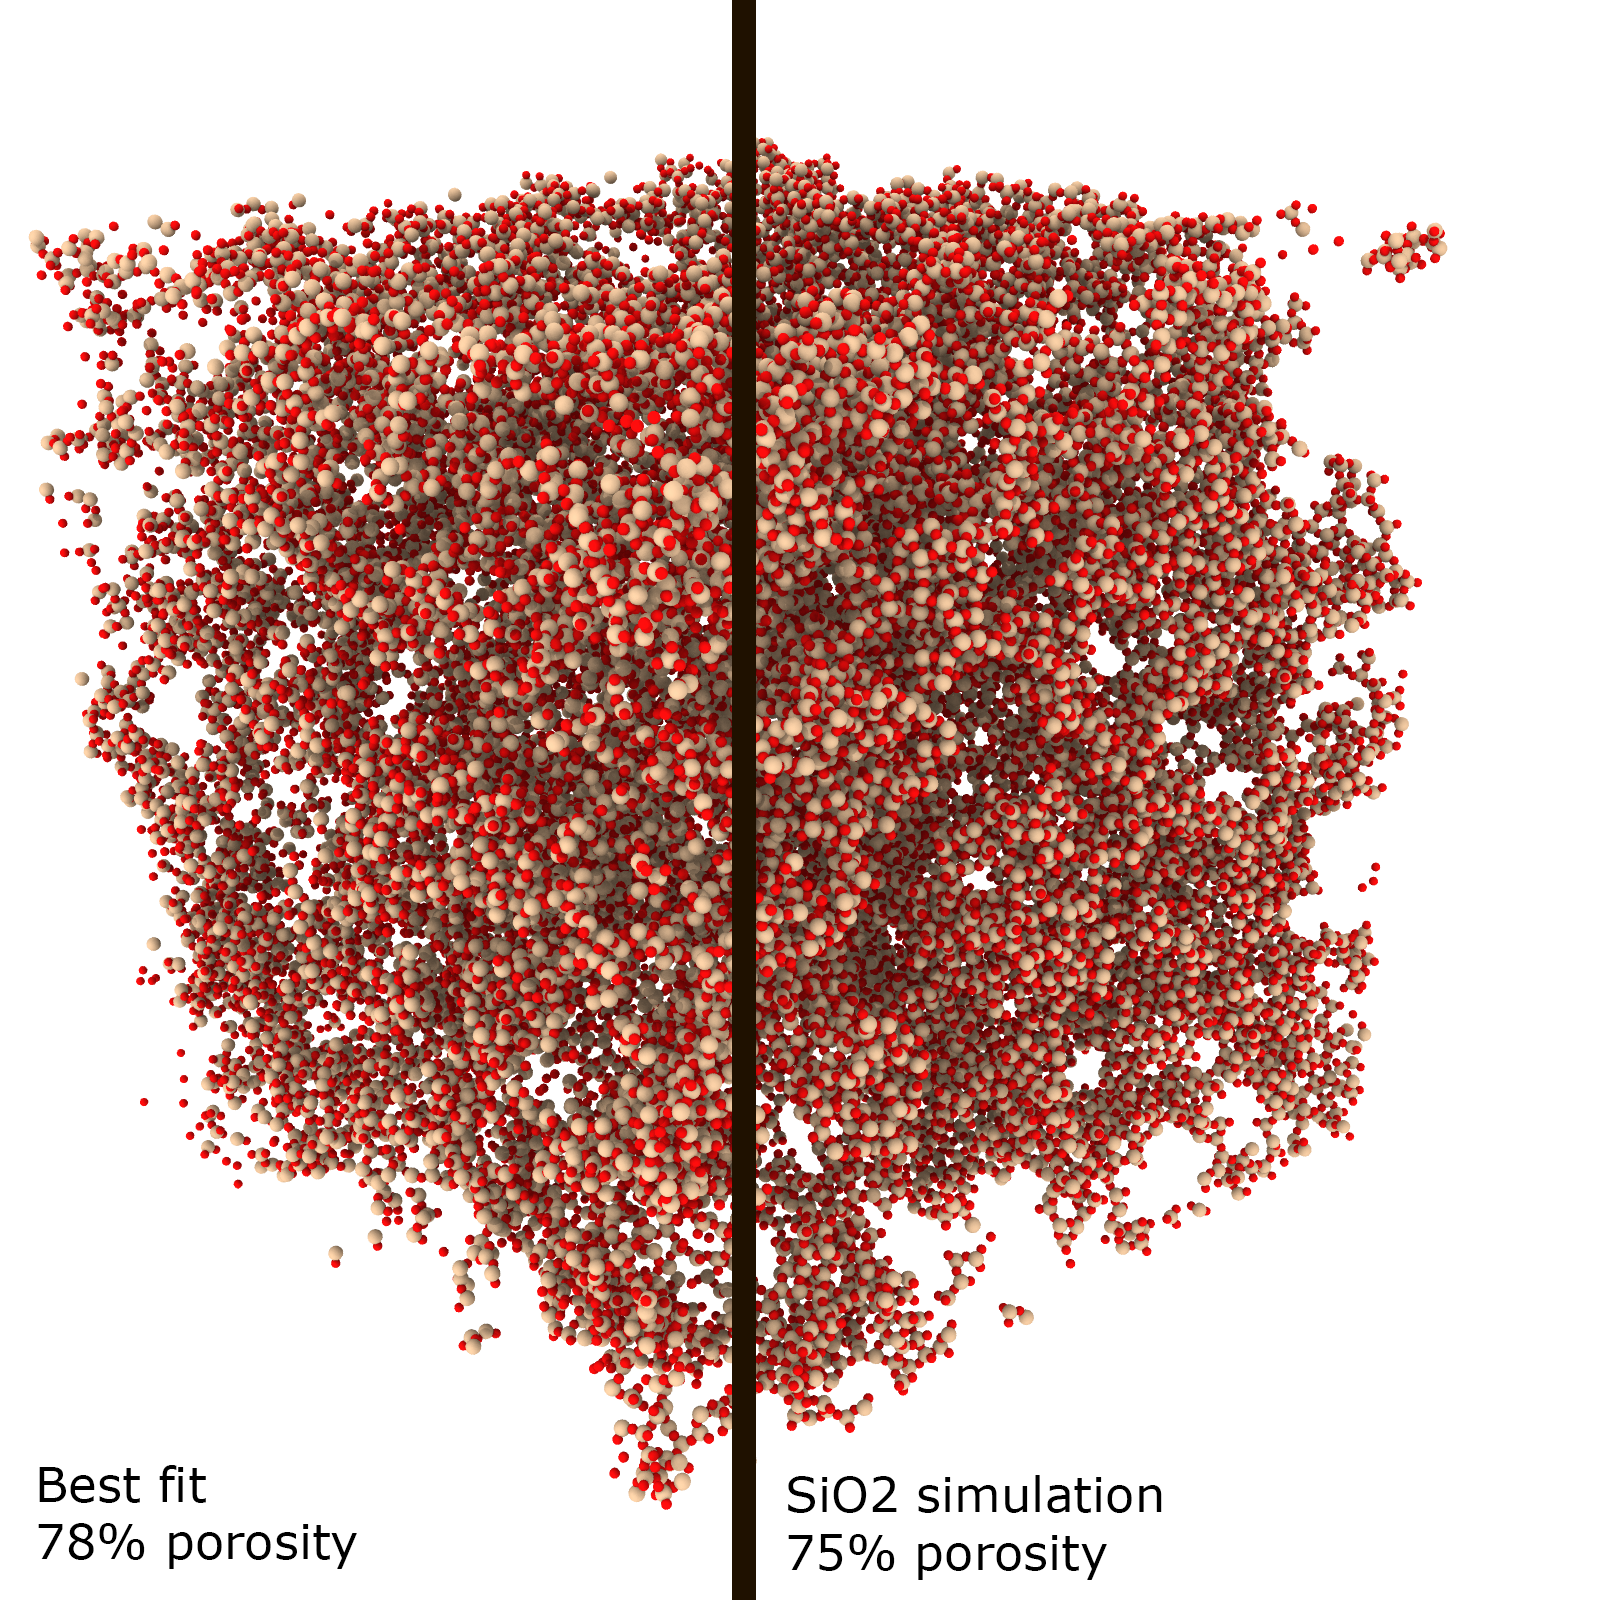
\includegraphics[width=.45\textwidth]{comparison.png}
\caption{Right side: A realisation of the best-fit parameters $\tau=-0.2$, $\psi=0.8$ and $\nu=0.3$.Left side: Simulated SiO$_2$ input data set used for parameter estimation. Although the pore geometry seems to be similar, we see some artifacts, such as single loose atoms in the generated geometry.}
\label{fig:porous_vs_model}
\end{figure}

The porosity of the input SiO$_2$ data set is $75\%$, while the best-fit data set has
porosity $77\% \pm 3 \%$, depending on the random seed. In addition, the surface area
of the original data set was $\sim \SI{29000}{\angstrom^2}$, while the best-fit data
shows similar values with surface are ranging between $\sim \SI{28000}{\angstrom^2}$ and $\sim \SI{30000}{\angstrom^2}$.
\todo{legg ved 3D plot av likelihood for aa vise at den er kjekk og fin}

\subsection{Discussion}
It is worth to note that since we are chiefly interested in obtaining a set of
parameters that reproduces a statistical correct representation of the input data,
we are relatively free to choose parameters as desired within the posterior distribution width of the parameter.
In the previous analysis, we selected a best fit threshold value of $\tau=-0.2$,
but from the width of the likelihood it is clear that nearby parameters would also be suitable. 
However, the surface area is strongly correlated with this value, so even slight
deviations (e.g. $\Delta \tau = 0.05$) yields a relatively large change in surface area. 
In addition, we do not claim that this model completely reproduces the pore structure
observed in nanoporous simulations, as is evident from the RDF shown in figure \ref{fig:gofr1},
but hope to discover a better model that will produce a $g(r)$ that is more in accordance with the data.

\subsection{$g(r)$ variation}
We also calculated the variation in the $g(r)$ given initial conditions on both our model and simulated data. 
In terms of the data, the variation is attributed as the initial velocities of the particles in the LAMMPS simulation. 
For the model, it corresponds to the random seed. We found that varying these
initial conditions have negligible effect on the calculation of $g(r)$.



\section{Conclusion}
\todo{konklusjon maa renskrives}

In this paper, we have proposed a novel method for generating a nanoporous media
using procedural methods in the form of simplex noise.
Procedural methods are not physical, but rather statistical models, and this gives
them some advatages over prevalent methods: they are computationally efficient, have low memory footprints and are only limited in terms of detail by the model in question. 
In particular, it is possible to create simulations of arbitrary scales and resolution, indeed with any level of detail. 

\todo{AMS: This is a bit weak currently. State first what you have succeeded in doing.
Then state the possible weaknesses of the model.}
We have developed a framework to generate nanoporous media using molecular dynamics simulations and
to estimate model parameters given such data. 
We have shown that it is possible through a full likelihood analysis to successfully reproduce the
input parameters of procedurally simulated data. 
In addition, we performed an analysis on a simulated $\SI{159}{\angstrom^{3}}$ data set of SiO$_2$,
and explain that while porosity and surface area correspond well between the model and data,
analysis of $g(r)$ shows that the current model reproduces the main features of the material, but that there are some deviations. 
We find the correspondence strong, which demonstrates the proof-of-principle of the use of
procedural noise methods, but we realize that even better correspondence may be achieved by
including other summations in the procedural noise modes. 

\subsection{Future work}
We have only considered the simplest kind of procedural noise: a simple sum over modes with
threshold cut-off $\tau$, scale fall-off persistence $\psi$ and initial scale $\nu$. 
We have also seen that, even through both porosity and surface area accurately reproduced,
there are features in the RDF that are not fully captured with the current model. 
This is evident from the images of the simulated structure seen in figure \ref{fig:porous_vs_model},
where the connecting nearly one-atom thin walls are difficult to reproduce with the current model. 
However, as procedural noise exert properties closely related to that of fractals, it is possible
to extend the number of parameters and define new models with very different properties. 
Some examples of these models are depicted in figure \ref{fig:future_models}, where the left- and
centre images show a new model with two new parameters (offset and gain), while the rightmost panel shows a simulation where the scale $\nu$ is itself being perturbed by procedural noise, yielding strong circular asymmetric patterns.   

Another immediate application would be to estimate model parameters given experimental observations of porous media. 
This would enable us to estimate new parameters such as instrumental noise, deviations from symmetry
(asymmetric properties), and pureness of samples. 
In addition, by analysing just a few samples and developing a model that produces similar structures
as in the specimens, we are able to produce an arbitrary amount of statistically correct samples,
free from instrumental noise and artefacts. 

A final key analysis would be to compare properties such as permeability through finite-element
simulations of gas/liquid flow through our simulated structures, in addition to exerting shear forces,
and comparing with actual simulated data from e.g. LAMMPS. 
Since the noise function is a continuous boolean function that only checks whether a position is
within a wall or void given a threshold, we are not limited to any size of the simulated system, and simulated particles traversing the media has arbitrary range.  

%Minkowski functionals and topology, genus etc

%Swiss noise

\begin{figure*}
\includegraphics[width=1\textwidth]{future_models.png}
\caption{Example of future models. Left panel: A multi-fractal model with thin surfaces and large pores. Centre panel: a multi fractal with cave-like structures. Right panel: A model with strong asymmetric noise. }
\label{fig:future_models}
\end{figure*}

%%%%%%%%%%%%%%%%%%%%%%%%%%%%%%%%%%%%%%%%%%%%%%%%%%%%%%%%%%%%%%
%%%%%%%%%%%%%%%%%%%%%%%%%%%%%%%%%%%%%%%%%%%%%%%%%%%%%%%%%%%%%%
\bibliography{bibliography}

\end{document}  